\documentclass[aspectratio=169]{beamer}

\usetheme{Boadilla}
\usefonttheme{professionalfonts}
\setbeamertemplate{navigation symbols}{}
\setbeamertemplate{itemize items}[circle]
\setbeamertemplate{enumerate items}[default]
\setbeamertemplate{headline}{}

\usepackage[utf8]{inputenc}
\usepackage[T1]{fontenc}
\usepackage{lmodern}
\usepackage{amsmath}
\usepackage{booktabs}
\usepackage{tabularx}
\usepackage{array}
\usepackage{hyperref}
\usepackage[strings]{underscore}
\usepackage{listings}
\usepackage{tikz}
\usetikzlibrary{arrows.meta,positioning,fit,calc,shapes.geometric}
\usepackage{xcolor}

\definecolor{courseblue}{HTML}{12355B}
\definecolor{coursegold}{HTML}{C98A2E}
\definecolor{courseice}{HTML}{EEF3F8}
\definecolor{coursegreen}{HTML}{2F6B4F}
\definecolor{coursegray}{HTML}{4B5563}
\definecolor{codebg}{HTML}{F7F9FC}
\definecolor{codecomment}{HTML}{5E6C84}
\definecolor{codestring}{HTML}{0B6E4F}

\setbeamercolor{palette primary}{bg=courseblue,fg=white}
\setbeamercolor{palette secondary}{bg=coursegold,fg=white}
\setbeamercolor{palette tertiary}{bg=courseblue,fg=white}
\setbeamercolor{palette quaternary}{bg=coursegold,fg=white}
\setbeamercolor{structure}{fg=courseblue}
\setbeamercolor{frametitle}{bg=courseice,fg=courseblue}
\setbeamercolor{title}{fg=courseblue}
\setbeamercolor{block title}{bg=courseblue,fg=white}
\setbeamercolor{block body}{bg=courseice,fg=black}
\setbeamercolor{normal text}{fg=black,bg=white}
\setbeamercolor{alerted text}{fg=coursegold}

\setbeamerfont{footline}{size=\scriptsize}

\setbeamertemplate{footline}{
  \leavevmode
  \hbox{
    \begin{beamercolorbox}[wd=.33\paperwidth,ht=2.8ex,dp=1.2ex,leftskip=0.8em]{palette primary}%
      University of Trieste
    \end{beamercolorbox}%
    \begin{beamercolorbox}[wd=.49\paperwidth,ht=2.8ex,dp=1.2ex,center]{palette tertiary}%
      \coursename{} \textbar{} \coursecode
    \end{beamercolorbox}%
    \begin{beamercolorbox}[wd=.18\paperwidth,ht=2.8ex,dp=1.2ex,rightskip=0.8em plus1fil]{palette secondary}%
      \insertframenumber{} / \inserttotalframenumber
    \end{beamercolorbox}%
  }
}

\hypersetup{
  colorlinks=true,
  linkcolor=courseblue,
  urlcolor=coursegreen
}

\lstdefinestyle{coursepython}{
  language=Python,
  basicstyle=\ttfamily\footnotesize,
  keywordstyle=\color{courseblue}\bfseries,
  commentstyle=\color{codecomment}\itshape,
  stringstyle=\color{codestring},
  showstringspaces=false,
  columns=fullflexible,
  keepspaces=true,
  frame=single,
  framerule=0.6pt,
  rulecolor=\color{courseblue},
  backgroundcolor=\color{codebg},
  xleftmargin=0.4em,
  xrightmargin=0.4em,
  aboveskip=0.4em,
  belowskip=0.2em
}

\newcommand{\coursename}{Data-driven Systems Engineering}
\newcommand{\coursecode}{440MI / 305SM}
\newcommand{\coursefooter}{}

\newcommand{\learninggoals}[1]{
  \begin{block}{Learning goals}
  #1
  \end{block}
}

\newcommand{\repoactivity}[1]{
  \begin{block}{Repo activity}
  #1
  \end{block}
}

\newcommand{\readinglist}[1]{
  \begin{block}{Papers and materials}
  {\footnotesize #1}
  \end{block}
}

\newcommand{\coursecontextframe}[5]{
  \begin{frame}{Course Map and Running Cases}
  \centering
  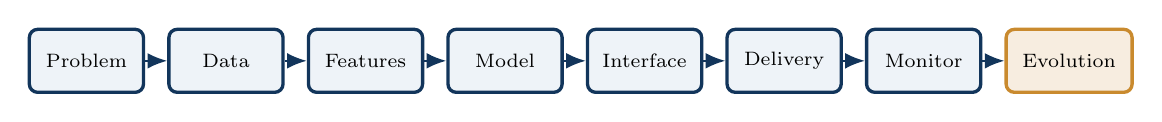
\begin{tikzpicture}[node distance=0.28cm]
  \node[flowbox, minimum width=1.45cm, minimum height=0.8cm] (problem) {\scriptsize Problem};
  \node[flowbox, minimum width=1.45cm, minimum height=0.8cm, right=of problem] (data) {\scriptsize Data};
  \node[flowbox, minimum width=1.45cm, minimum height=0.8cm, right=of data] (features) {\scriptsize Features};
  \node[flowbox, minimum width=1.45cm, minimum height=0.8cm, right=of features] (model) {\scriptsize Model};
  \node[flowbox, minimum width=1.45cm, minimum height=0.8cm, right=of model] (interface) {\scriptsize Interface};
  \node[flowbox, minimum width=1.45cm, minimum height=0.8cm, right=of interface] (delivery) {\scriptsize Delivery};
  \node[flowbox, minimum width=1.45cm, minimum height=0.8cm, right=of delivery] (monitor) {\scriptsize Monitor};
  \node[accentbox, minimum width=1.6cm, minimum height=0.8cm, right=of monitor] (evolution) {\scriptsize Evolution};
  \foreach \a/\b in {problem/data,data/features,features/model,model/interface,interface/delivery,delivery/monitor,monitor/evolution} {
    \draw[arrow] (\a) -- (\b);
  }
  \end{tikzpicture}

  \vspace{0.5em}
  \begin{block}{Today in the course}
  \textbf{Focus:} #1

  \textbf{Bridge:} #2
  \end{block}

  \begin{columns}[T]
  \column{0.48\textwidth}
  \begin{block}{Fraud case}
  {\footnotesize #3}
  \end{block}
  \column{0.48\textwidth}
  \begin{block}{Pasteurization case}
  {\footnotesize #4}
  \end{block}
  \end{columns}

  \vspace{0.3em}
  {\footnotesize \textbf{Course thread:} #5}
  \coursefooter
  \end{frame}
}

\newcommand{\classclosingframe}[4]{
  \begin{frame}{From This Class to the Next}
  \begin{block}{What stays with us}
  #1
  \end{block}

  \begin{columns}[T]
  \column{0.48\textwidth}
  \begin{block}{Project use}
  {\footnotesize #2}
  \end{block}
  \column{0.48\textwidth}
  \begin{block}{Next connection}
  {\footnotesize #3}
  \end{block}
  \end{columns}

  \vspace{0.3em}
  {\footnotesize \textbf{Course thread:} #4}
  \coursefooter
  \end{frame}
}

\tikzset{
  flowbox/.style={
    rounded corners=3pt,
    draw=courseblue,
    fill=courseice,
    very thick,
    minimum width=2.2cm,
    minimum height=0.9cm,
    align=center,
    font=\small
  },
  accentbox/.style={
    rounded corners=3pt,
    draw=coursegold,
    fill=coursegold!15,
    very thick,
    minimum width=2.2cm,
    minimum height=0.9cm,
    align=center,
    font=\small
  },
  arrow/.style={
    -{Latex[length=2.5mm,width=2mm]},
    thick,
    draw=courseblue
  }
}


\title{Class 25: Requirements Engineering in Practice}
\subtitle{Session 25 of 36 -- Hands-on Workshop}
\author{\coursename}
\date{}

\begin{document}

\frame{\titlepage \coursefooter}

\begin{frame}{Agenda}
\begin{itemize}
\item Recap: what makes a requirement good
\item Workshop structure and case assignment
\item Elicitation: asking the right questions
\item Writing functional and non-functional requirements
\item Surfacing conflicts and trade-offs
\item Peer review against a validation checklist
\end{itemize}
\coursefooter
\end{frame}

\begin{frame}{From theory to a written specification}
\learninggoals{
\begin{itemize}
\item Apply elicitation techniques to a concrete case in one working session.
\item Draft testable functional and non-functional requirements from a vague prompt.
\item Identify a genuine conflict between requirements and propose an explicit trade-off.
\item Use a validation checklist to critique a peer team's requirements.
\end{itemize}
}
\coursefooter
\end{frame}

\coursecontextframe
{Turning requirements theory into a written, testable specification.}
{This session applies Class 23's theory, sharpened by YesAlps' real-world session in Class 24, to a hands-on writing exercise instead of another lecture.}
{Fraud track: write functional and non-functional requirements for the fraud scoring service, from ingestion to analyst review.}
{Pasteurization track: write functional and non-functional requirements for the abnormal-state alerting dashboard.}
{Requirements written today should be traceable to the tests, deployment gates, and monitoring rules the course covers later.}

\begin{frame}{Recap: qualities of a good requirement}
\begin{itemize}
\item Necessary, testable, unambiguous, feasible, traceable.
\item A requirement is not a feature wish; it is something a reviewer could check.
\end{itemize}
\begin{block}{Weak versus better, one more time}
``The system should be reliable'' versus ``the stream endpoint shall recover and resume within 5 seconds after a dropped connection.''
\end{block}
\coursefooter
\end{frame}

\begin{frame}{Workshop structure}
\begin{itemize}
\item Form small groups; each group picks one track: fraud scoring or pasteurization alerting.
\item Time-box each stage; a rough spec beats an unfinished perfect one.
\item Every stage below produces a short written artifact the group keeps.
\end{itemize}
\begin{enumerate}
\item Elicit (10 min)
\item Draft functional requirements (10 min)
\item Draft non-functional requirements (10 min)
\item Surface one conflict (5 min)
\item Peer review with the checklist (10 min)
\end{enumerate}
\coursefooter
\end{frame}

\begin{frame}{Elicitation is structured discovery}
\begin{itemize}
\item Elicitation means discovering requirements from users, operators, policies, data constraints, and business goals.
\item Interviews, observation, document review, and prototype walkthroughs are all useful methods.
\item The purpose is not only to collect wishes, but to reveal conflicts and hidden assumptions.
\end{itemize}
\coursefooter
\end{frame}

\begin{frame}{Good elicitation prompts for project teams}
\begin{itemize}
\item Who acts on the prediction, and what action do they take?
\item What happens if the model is unavailable for one hour?
\item Which inputs may arrive late, missing, or malformed?
\item When do labels appear, and who trusts them?
\item Which requirement is actually a policy or compliance constraint?
\end{itemize}
\coursefooter
\end{frame}

\begin{frame}{Exercise 1: Elicitation notes}
\begin{itemize}
\item Answer the prompts on the previous slide for your chosen track.
\item Write raw notes, not polished sentences; contradictions between teammates are useful signal, not noise.
\item Flag anything that sounds like a policy or domain constraint rather than a feature request.
\end{itemize}
\coursefooter
\end{frame}

\begin{frame}{From notes to functional requirements}
\begin{block}{Raw note}
``The analyst needs to know why a transaction was flagged.''
\end{block}
\begin{block}{Functional requirement}
The API shall return, alongside the score, the top 3 contributing features for each flagged transaction.
\end{block}
\begin{itemize}
\item A functional requirement names an observable system behavior, not a feeling.
\end{itemize}
\coursefooter
\end{frame}

\begin{frame}{Exercise 2: Write three functional requirements}
\begin{itemize}
\item Using your elicitation notes, write three functional requirements for your track.
\item Each one should name an input, an action, and an observable output.
\item Avoid the words ``should'' and ``easy''; prefer ``shall'' plus a concrete behavior.
\end{itemize}
\coursefooter
\end{frame}

\begin{frame}{Non-functional requirements deserve equal weight}
\begin{tabularx}{\textwidth}{>{\bfseries}l X}
Category & Question to answer with a number \\
\toprule
Latency & How fast must a response or alert be, and for what fraction of cases? \\
Availability & How much downtime is tolerable, and what happens during it? \\
Auditability & What must be logged, and for how long? \\
Privacy & What data can be stored, shown, or shared, and with whom? \\
\bottomrule
\end{tabularx}
\coursefooter
\end{frame}

\begin{frame}{Exercise 3: Write two non-functional requirements}
\begin{itemize}
\item Pick two categories from the table and write one requirement each.
\item Every requirement must include a number: a time, a percentage, a retention period, or a rate.
\item If you cannot put a number on it yet, write down what you would need to know to add one.
\end{itemize}
\coursefooter
\end{frame}

\begin{frame}{Conflicts between requirements are normal}
\begin{itemize}
\item Fast response may conflict with more detailed explanations.
\item High recall may conflict with low false positive rates.
\item Privacy constraints may limit what data can be stored for monitoring or audit.
\item Requirements engineering helps teams make these trade-offs explicit.
\end{itemize}
\coursefooter
\end{frame}

\begin{frame}{Exercise 4: Name one conflict}
\begin{itemize}
\item Look at your functional and non-functional requirements together.
\item Find one real tension between them, for example explanation detail versus latency.
\item Write one sentence stating which side you would favor by default, and why.
\end{itemize}
\coursefooter
\end{frame}

\begin{frame}{Validation techniques that fit student projects}
\begin{itemize}
\item Requirement reviews with a checklist for ambiguity and measurability.
\item Use-case walkthroughs for edge cases and operator behavior.
\item Prototype validation with a minimal dashboard or API client.
\item Acceptance test drafting before full implementation.
\end{itemize}
\coursefooter
\end{frame}

\begin{frame}{Exercise 5: Peer review}
\begin{itemize}
\item Swap your written requirements with another group.
\item For each requirement, check: necessary, testable, unambiguous, feasible, traceable.
\item Mark anything that fails a check and suggest a one-line fix.
\end{itemize}
\coursefooter
\end{frame}

\begin{frame}{Ground your requirement in something real}
\repoactivity{
\begin{itemize}
\item Fraud track: anchor requirements to the fields the API already accepts and returns, as seen in `Class6_model_api.py`.
\item Pasteurization track: anchor requirements to the fields already streamed by `pasteurization/serving.py`, such as state, T, pH, and dTdt.
\item A requirement that cannot be tied to an existing field or endpoint is either a new feature request or still too vague.
\end{itemize}
}
\coursefooter
\end{frame}

\begin{frame}{Discussion prompt}
\begin{block}{Question}
Which of your non-functional requirements would be hardest to test automatically, and why?
\end{block}
\begin{itemize}
\item This surfaces the gap between writing a requirement and actually verifying it.
\item It is a preview of the testing and monitoring gates later in the course.
\end{itemize}
\coursefooter
\end{frame}

\begin{frame}{What a strong requirements artifact looks like}
\begin{itemize}
\item A short list of functional requirements naming input, action, and output.
\item A short list of non-functional requirements, each with a number attached.
\item At least one documented conflict and the team's default resolution.
\item Peer-review marks showing the requirements survived a second reading.
\end{itemize}
\coursefooter
\end{frame}

\begin{frame}{Papers and materials}
\readinglist{
\href{https://www.pearson.com/en-us/subject-catalog/p/software-engineering/P200000003144/9780137035151}{Sommerville, Software Engineering};\
\href{https://ieeexplore.ieee.org/document/720574}{IEEE recommended practice for software requirements specifications};\
\href{https://www.atlassian.com/agile/project-management/user-stories}{User stories and acceptance criteria guide};\
\href{https://www.altexsoft.com/blog/functional-and-non-functional-requirements-specification-and-types/}{Practical overview of functional and non-functional requirements}.
}
\coursefooter
\end{frame}

\classclosingframe
{\begin{itemize}
\item A requirement earns its place only if someone could check whether it was met.
\item Elicitation, drafting, and peer review are fast enough to run in a single session.
\item Conflicts between requirements are normal and should be written down, not hidden.
\end{itemize}}
{Keep today's written requirements; they are the seed of the project proposal work in Class 32 and Class 34.}
{Class 26 moves from what the system must do to how the team organizes work to build it, starting with process models and agile foundations.}
{Today's artifact is the first concrete deliverable in the course thread that eventually becomes each team's own project.}

\end{document}
